\section{W2: Domain models, SSDs}

\subsection{Domain class diagram}
A static model with conceptual classes that represent real-situations, and has associations and attributes but not methods.
\textbf{Generalisation-specialisation class hierarchy:} a class that is a generalisation of other classes, and has subclasses that are specialisations of the generalisation.\\
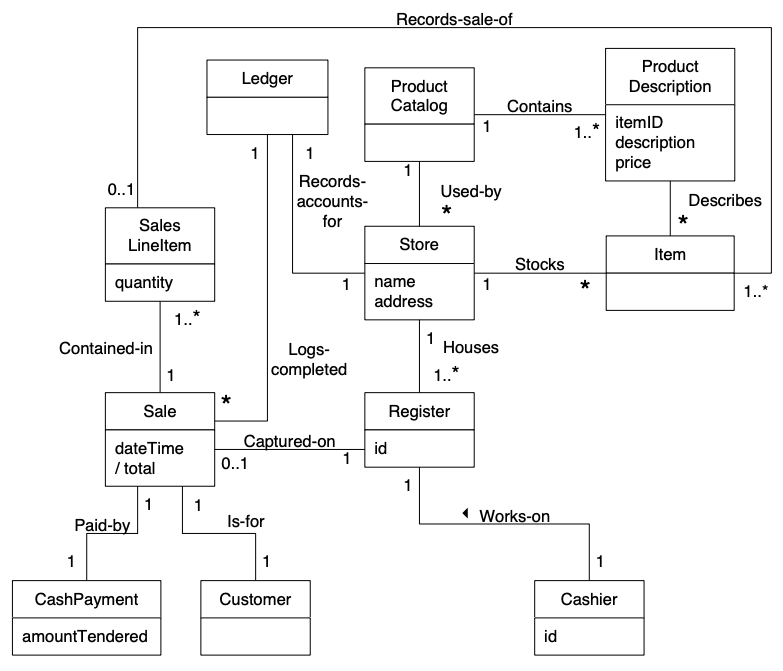
\includegraphics[width=\linewidth]{figs/domain-model.png}

\subsection{System sequence diagrams}
A dynamic model of context in a system. It shows the interactions between actors and the system, and the order of messages.\\
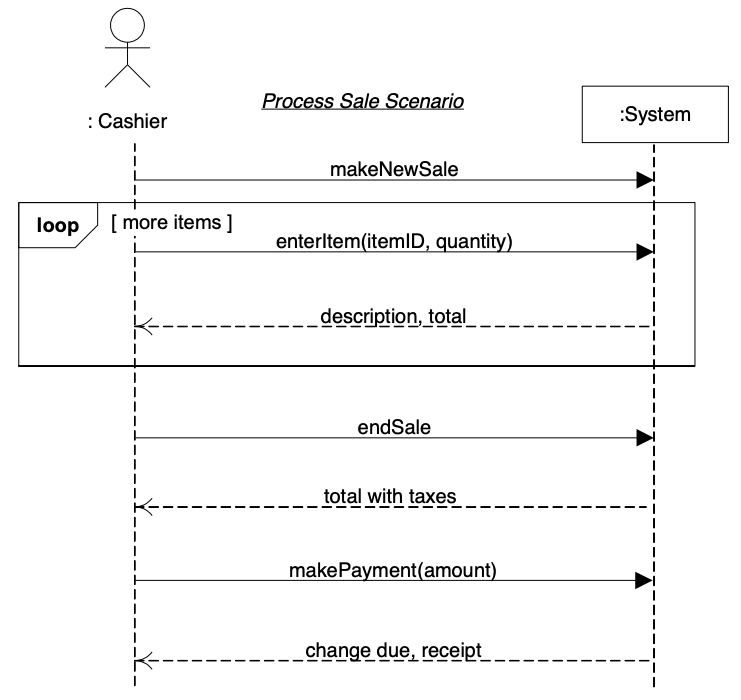
\includegraphics[width=\linewidth]{figs/system-sequence-diagram.png}
